\documentclass[a4paper, 12pt]{article}
\usepackage[]{cite}
\usepackage{cmap}
\usepackage[T2A]{fontenc}
\usepackage[utf8]{inputenc}
\usepackage[english, russian]{babel}
\usepackage{amsmath,amsfonts,amssymb,amsthm,mathtools,dsfont}
\usepackage{icomma}
\usepackage[dvips]{graphicx}
\usepackage{epsfig}
\usepackage{extsizes}
\usepackage{subfig}
\usepackage{color}
\usepackage{enumitem}
\usepackage{hyperref}
\usepackage{tabularx}
\usepackage[square,sort,comma,numbers]{natbib}

\hypersetup{
	colorlinks=true,
	linkcolor=blue,
	urlcolor=cyan,
}

\newcommand\argmin{\mathop{\arg\min}}
\newcommand{\hchi}{\hat{\boldsymbol{\chi}}}
\newcommand{\hphi}{\hat{\boldsymbol{\varphi}}}
\newcommand{\bchi}{\boldsymbol{\chi}}
\newcommand{\A}{\mathcal{A}}
\newcommand{\B}{\mathcal{B}}
\newcommand{\x}{\mathbf{x}}
\newcommand{\hx}{\hat{x}}
\newcommand{\hy}{\hat{y}}
\newcommand{\M}{\mathcal{M}}
\newcommand{\N}{\mathcal{N}}
\newcommand{\R}{\mathbb{R}}
\newcommand{\p}{p(\cdot)}
\newcommand{\q}{q(\cdot)}
\newcommand{\uu}{\mathbf{u}}
\newcommand{\vv}{\mathbf{v}}
\newcommand{\bz}{\mathbf{z}}
\newcommand{\bx}{\mathbf{x}}
\newcommand{\by}{\mathbf{y}}
\newcommand{\bv}{\mathbf{v}}
\newcommand{\bw}{\mathbf{w}}
\newcommand{\ba}{\mathbf{a}}
\newcommand{\bb}{\mathbf{b}}
\newcommand{\bff}{\mathbf{f}}
\newcommand{\bh}{\mathbf{h}}
\newcommand{\bl}{\mathbf{l}}
\newcommand{\bp}{\mathbf{p}}
\newcommand{\bq}{\mathbf{q}}
\newcommand{\bs}{\mathbf{s}}
\newcommand{\bt}{\mathbf{t}}
\newcommand{\bu}{\mathbf{u}}
\newcommand{\bT}{\mathbf{T}}
\newcommand{\bX}{\mathbf{X}}
\newcommand{\bZ}{\mathbf{Z}}
\newcommand{\bS}{\mathbf{S}}
\newcommand{\bH}{\mathbf{H}}
\newcommand{\bW}{\mathbf{W}}
\newcommand{\bY}{\mathbf{Y}}
\newcommand{\bU}{\mathbf{U}}
\newcommand{\bQ}{\mathbf{Q}}
\newcommand{\bP}{\mathbf{P}}
\newcommand{\bA}{\mathbf{A}}
\newcommand{\bB}{\mathbf{B}}
\newcommand{\bC}{\mathbf{C}}
\newcommand{\bE}{\mathbf{E}}
\newcommand{\bF}{\mathbf{F}}
\newcommand{\bsigma}{\boldsymbol{\sigma}}
\newcommand{\bomega}{\boldsymbol{\omega}}
\newcommand{\btheta}{\boldsymbol{\theta}}
\newcommand{\bgamma}{\boldsymbol{\gamma}}
\newcommand{\bdelta}{\boldsymbol{\delta}}
\newcommand{\bPsi}{\boldsymbol{\Psi}}
\newcommand{\bpsi}{\boldsymbol{\psi}}
\newcommand{\bxi}{\boldsymbol{\xi}}
\newcommand{\bmu}{\boldsymbol{\mu}}
\newcommand{\bzeta}{\boldsymbol{\zeta}}
\newcommand{\blambda}{\boldsymbol{\lambda}}
\newcommand{\beps}{\boldsymbol{\varepsilon}}
\newcommand{\bZeta}{\boldsymbol{Z}}
% mathcal
\newcommand{\cX}{\mathcal{X}}
\newcommand{\cY}{\mathcal{Y}}
\newcommand{\cW}{\mathcal{W}}

\newcommand{\dH}{\mathds{H}}
\newcommand{\dR}{\mathds{R}}
% transpose
\newcommand{\T}{^{\mathsf{T}}}

% command to strike out text
\newcommand{\stkout}[1]{\ifmmode\text{\sout{\ensuremath{#1}}}\else\sout{#1}\fi}

\renewcommand{\epsilon}{\ensuremath{\varepsilon}}
\renewcommand{\phi}{\ensuremath{\varphi}}
\renewcommand{\kappa}{\ensuremath{\varkappa}}
\renewcommand{\le}{\ensuremath{\leqslant}}
\renewcommand{\leq}{\ensuremath{\leqslant}}
\renewcommand{\ge}{\ensuremath{\geqslant}}
\renewcommand{\geq}{\ensuremath{\geqslant}}
\renewcommand{\emptyset}{\varnothing}


\renewcommand{\baselinestretch}{1}


\newtheorem{Th}{Теорема}
\newtheorem{Def}{Определение}
\newenvironment{Proof} % имя окружения
{\par\noindent{\bf Доказательство.}} % команды для \begin
{\hfill$\scriptstyle\blacksquare$} % команды для \end
\newtheorem{Assumption}{Предположение}
\newtheorem{Corollary}{Следствие}
\newtheorem{problem}{Problem}


\textheight=24cm % высота текста
\textwidth=16cm % ширина текста
\oddsidemargin=0pt % отступ от левого края
\topmargin=-1.5cm % отступ от верхнего края
\parindent=24pt % абзацный отступ
\parskip=0pt % интервал между абзацами
\tolerance=2000 % терпимость к "жидким" строкам
\flushbottom % выравнивание высоты страниц

\graphicspath{{../figures/}}



\begin{document}
	
	\thispagestyle{empty}
	\begin{center}
		\sc
		Министерство образования и науки Российской Федерации\\
		Московский физико-технический институт
		{\rm(государственный университет)}\\
		Физтех-школа прикладной математики и информатики\\
		Кафедра <<Интеллектуальные системы>>\\[35mm]
		\rm\large
		Владимиров Эдуард Анатольевич\\[10mm]
		\bf\Large
		Модели пространства состояний в задачах классификации сигналов ЭКоГ \\[10mm]
		\rm\normalsize
		010990 --- Интеллектуальный анализ данных\\[10mm]
		\sc
		Выпускная квалификационная работа бакалавра\\[10mm]
	\end{center}
	\hfill\parbox{80mm}{
		\begin{flushleft}
			\bf
			Научный руководитель:\\
			\rm
			д.~ф.-м.~н. Стрижов Вадим Викторович\\[5cm]
		\end{flushleft}
	}
	\begin{center}
		Москва\\
		2023
	\end{center}
	
	\newpage
	\tableofcontents
	\newpage
	
	\begin{abstract}
		Данная работа посвящена нейронному декодированию ~--- восстановлению стимула по сигналам головного мозга. А именно, рассматривается задача бинарной классификации сигналов, полученных во время движения руки. Для получения высокого качества классификации предлагается использовать модели глубокого обучения. В задаче декодирования сигналов часто применяются свёрточные нейронные сети и трансформеры, в то время как модели пространства состояний применяются редко. Предлагается восполнить данный пробел и подготовить практическое руководство к выбору модели из данного семейства. Проведено сравнение следующих моделей пространства состояний: RNN, NCDE, S4. Для анализа качества алгоритмов предсказания проводится вычислительный эксперимент на данных ЭКоГ.
		
		\bigskip
		\textbf{Ключевые слова}: \emph{ЭКоГ, нейронное декодирование, модели пространства состояний, RNN, S4, NCDE}
	\end{abstract}
	
	\newpage
	
	%%%%%%%%%%%%%%%%%%%%%%%%%%%%%%%%%%%%%%%%%%%%%%%%%%%%%%%%%%%%%%%%%%%%%%%%%%%%%%%%%%%%%%%%%%%%%%%%%%%%%%%%%%%%%%%%%%%%%%%%%%%%%%%%%%
	\section{Введение}
	
	Нейронное декодирование ~-- процесс расшифровки информации, полученной в результате нейронной активности ~-- имеет большие перспективы в понимании сложностей человеческого мозга и разработке передовых приложений в таких областях, как нейропротезирование и интерфейсы мозг-компьютер.
	Нейронное декодирование включает в себя извлечение значимой информации из данных об активности головного мозга с целью вывода когнитивных состояний, намерений движения или ощущений.
	Например, исследователи предсказывают движения, основываясь на активности в моторной коре \citep{temp_ethier2012restoration}, действия, основанные на активности в префронтальной и теменной коре \citep{temp_ibos2017sequential}, и пространственные местоположения, основанные на активности в гиппокампе \citep{temp_davidson2009hippocampal}. 
	%Эти расшифрованные предсказания могут быть использованы для управления устройствами(например, роботизированной конечностью) или для лучшего понимания того, как области мозга соотносятся с внешним миром.
	Расшифровывание сигналов головного мозга даёт нам понять, как мозг обрабатывает и представляет информацию о мире, открывая путь к революционным достижениям в понимании и взаимодействии с мозгом.

	По сути, нейронное декодирование - это задача классификации (или регрессии), связывающая нейронные сигналы с определенными переменными. 
	При такой постановке проблемы становится очевидным, что существует широкий спектр методов, которые можно применить. 
	Однако, несмотря на недавние достижения в области методов глубокого обучения, по-прежнему принято декодировать сигналы традиционным подходом.
	Этот подход включает в себя фильтрацию сигналов от шума, извлечение временных, частотных, пространственных и статистических признаков и применение классического алгоритма машинного обучения, будь то логистическая регрессия, метод опорных векторов или линейный дискриминантный анализ \citep{firuzi2022decoding}.
	Использование современных алгоритмов машинного обучения позволяет значительно повысить качество прогноза.
	Стоит отметить, что модели глубокого обучения применяются не только при прогнозировании, но и для предобработки данных от шума.
	Для этого используются свёрточные автоэнкодеры \citep{temp_leite2018deep, temp_caldas2020towards} и генеративно-состязательные сети \citep{temp_an2022auto}.
	
	В области нейронного декодирования широкое распространение получили свёрточные нейронные сети \citep{eegnet, htnet} и трансформеры \citep{defossez2022decoding, tang2023semantic}.
	В то же время как модели пространства состояний (SSM) используются исключительно в байесовском ключе, будь то фильтр Калмана \citep{kalman1961}, скрытые марковские цепи \citep{paninski2010new} или линейная модель со скрытыми состояниями \citep{wu2009neural}.
	То есть, с точки зрения глубокого обучения модели пространства состояний практически не применяются в рассматриваемой задаче.
	Хотя они дают математическую основу для моделирования сложной динамики нейронных систем.
	Поэтому, предлагается заполнить этот пробел, применив глубокие нейронные сети, относящиеся к SSM, в задаче нейронного декодирования.
	
	Выбор соответствующей модели является важным, поскольку различные алгоритмы обладают отличительными характеристиками, которые могут значительно влиять на конечный результат.
	Поэтому крайне важно тщательно изучить и сравнить свойства моделей, чтобы предоставить практическое руководство по их выбору. 
	Понимая сильные и слабые стороны каждой из них, исследователи и практики смогут принимать обоснованные решения при разработке экспериментов и приложений в области нейронного декодирования.
	
	В данной работе рассматриваются следующие модели пространства состояний: рекуррентные нейронные сети (RNN) \citep{rnn}, нейронные контролируемые дифференциальные уравнения (NCDE) \citep{ncde}, модель структурного пространства состояний (S4) \citep{s4}.
	
	Таким образом, основной вклад работы заключается в рассмотрении моделей пространства состояний в задаче нейронного декодирования и представлении рекомендации по их применению на основе свойств перечисленных выше моделей.
	
	Остальная часть работы организована следующим образом. Раздел 2 раскрывает смысл используемых обозначений. Раздел 3 даёт формальную постановку решаемой задачи. Раздел 4 представляет обзор литературы по применению моделей пространства состояний в задаче нейронного декодирования. Раздел 5 представляет подробный анализ и сравнение моделей RNN, S4 и NCDE. Раздел 6 предоставляет практическое руководство по выбору модели пространства состояний, полученное на основе вычислительного эксперимента. Наконец, раздел 7 завершает работу, подчеркивая её вклад.
	
	%%%%%%%%%%%%%%%%%%%%%%%%%%%%%%%%%%%%%%%%%%%%%%%%%%%%%%%%%%%%%%%%%%%%%%%%%%%%%%%%%%%%%%%%%%%%%%%%%%%%%%%%%%%%%%%%%%%%%%%%%%%%%%%%
	\section{Обозначения}
	
	\begin{itemize}
		\item[] ЭКоГ ~--- электрокортикограмма
		\item[] RNN ~--- Recurrent Neural Network
		\item[] CNN ~--- Convolutional Neural Network
		\item[] S4 ~--- Structured State Space for Sequence Modeling
		\item[] NODE/Neural ODE ~--- Neural Ordinary Differential Equation
		\item[] NCDE/Neural CDE ~--- Neural Controlled Differential Equation
		\item[] SSM ~--- State Space Models
		\item[] МКР ~--- межквартильный размах
	\end{itemize}
	
	%%%%%%%%%%%%%%%%%%%%%%%%%%%%%%%%%%%%%%%%%%%%%%%%%%%%%%%%%%%%%%%%%%%%%%%%%%%%%%%%%%%%%%%%%%%%%%%%%%%%%%%%%%%%%%%%%%%%%%%%%%%%%%%
	\section{Постановка задачи классификации сигнала ЭКоГ}
	
	Пусть $\bX \in \dR^{M \times N \times T}$ ~--- $M$ измерений ЭКГ, где $N$ ~--- число электродов, $T$ ~--- число элементов временного ряда. Одному измерению ЭКГ соответствуют набор сигналов, записанный на некоторый промежуток времени, во время которого был совершён некий стимул.
	
	$Y \in \{ 0, 1\}^M$ ~--- целевая переменная, индикатор наличия/отсутствия стимула.
	
	Целевая функция $ \bff: \bX \times W \to Y$, где $W \in \dR^P$ ~--- параметры модели
	
	Критерий качества ~--- бинарная кросс-энтропия с $L2$-регуляризацией:  
	
	$$ L(\bw) = -\dfrac{1}{M} \sum\limits_{m=1}^M y_m \log(f(\bw, \bx)) + (1 - y_m) \log(1 - f(\bw, \bx)) + \lambda ||\bw||^2$$
	
	Оптимизационная задача ~--- выбор модели, доставляющей минимум критерия качества: $$\hat{\bw} = \underset{\bw}{\arg \min} \; L(\bw)$$
	
	Основная метрика для этой задачи ~-- точность (accuracy), поскольку классы сбалансированы.
	%%%%%%%%%%%%%%%%%%%%%%%%%%%%%%%%%%%%%%%%%%%%%%%%%%%%%%%%%%%%%%%%%%%%%%%%%%%%%%%%%%%%%%%%%%%%%%%%%%%%%%%%%%%%%%%%%%%%%%%%%%%%%%%%%%%%%%%
	\section{Обзор существующих подходов к декодированию сигналов}
	Основная задача данной работы ~--- анализ свойств моделей пространства состояний на примере задачи классификации сигналов ЭКоГ на два класса ~--- "движение" и "покой". 
	
	На данный момент классический подход выглядит следующим образом: сигнал фильтруется для удаления шумов, затем применяются преобразования для извлечения признаков (среднее и максимум, параметры Хёрша, вейвлет-преобразование, преобразование Фурье или преобразование Гильберта). После этого применяется алгоритм классификации (логистическая регрессия, метод опорных векторов, наивный байесовский классификатор или линейный дискриминантный анализ).
	
	С ростом популярности глубоких нейронных сетей появился новый подход, в котором нейронные сети берут на себя и генерацию признаков, и процесс предсказания.
	В работе \citep{xie2018decoding} в задаче декодирования движения пальца по данным ЭКоГ использовался гибридный подход: CNN отвечала за извлечение признаков, а RNN отвечал за распознание временной динамики.
	В работе \citep{wang2018ajile} также использовалась связка CNN + RNN для определения движения суставов верхней части тела, основанную как на данных ЭКоГ, так и на видеоданных
	В работе \citep{du2018decoding} использовались рекуррентные нейронные сети, которые распознавали временные зависимости в сигналах ЭКоГ для быстрого декодирования жестов.
	
	Таким образом, в глубоких сетях из моделей пространства состояний используется только RNN и её модификации (LSTM, GRU).
	
	Существует ещё один подход ~--- иерархический. В нём объединено несколько алгоритмов и цепочек обработки, которые выполняют переключение или регулировку весов. Применяется в задачах с сигналами, поступающими в реальном времени.
	
	Иллюстрация вышеперечисленных подходов приведена на рисунке \ref{fig:ecog-approaches}
	
	\begin{figure}[bhtp]
		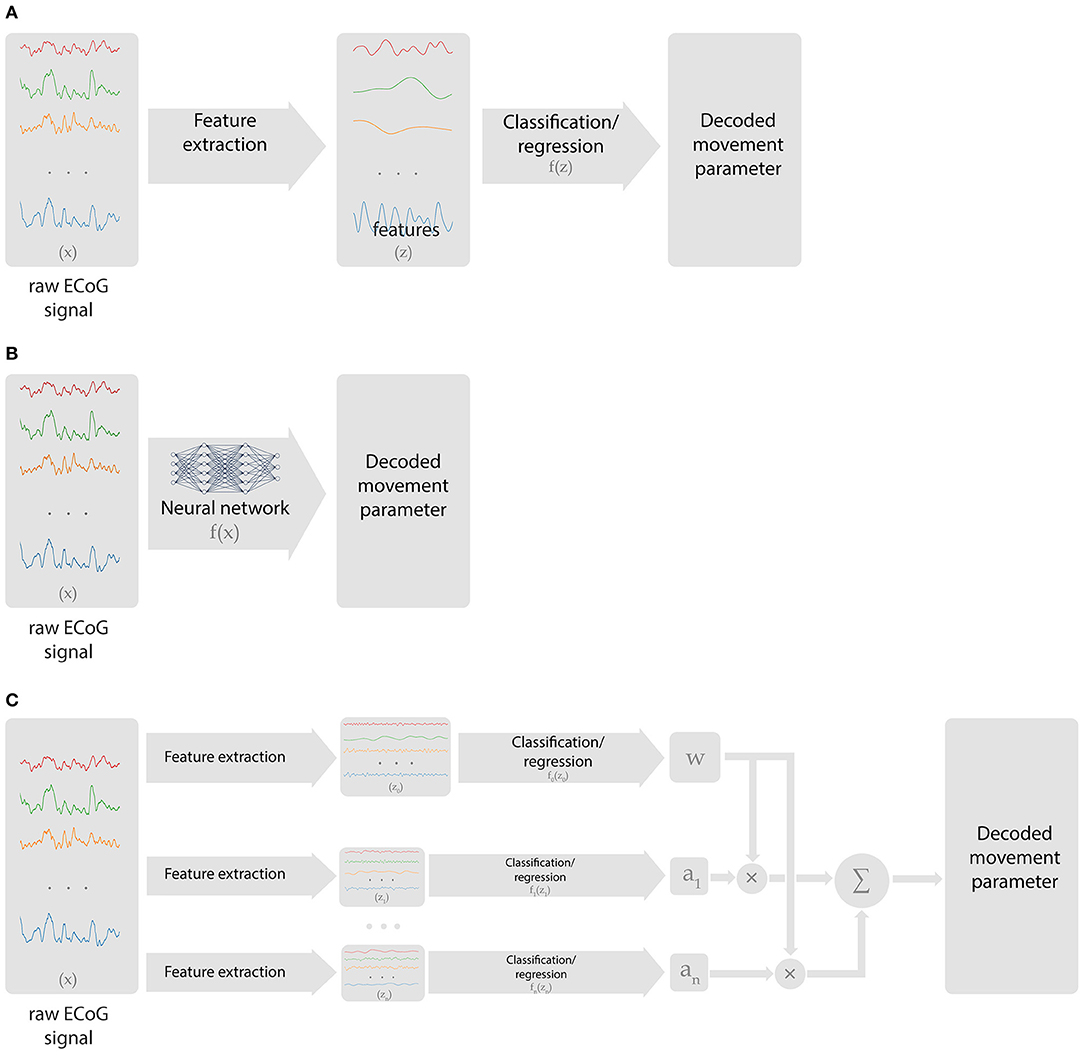
\includegraphics[width=\textwidth]{ecog-decoding-approaches.jpg}
		\caption{Подходы к работе с данными ЭКоГ. \textbf{(A)} Классический подход. \textbf{(B)} Подход глубокого обучения. \textbf{(C)} Ансамбль моделей. Взято из \citep{volkova2019decoding}}
		\label{fig:ecog-approaches}
	\end{figure}
		
	%%%%%%%%%%%%%%%%%%%%%%%%%%%%%%%%%%%%%%%%%%%%%%%%%%%%%%%%%%%%%%%%%%%%%%%%%%%%%%%%%%%%%%%%%%%%%%%%%%%%%%%%%%%%%%%%%%%%%%%%%%%%%%%%%%%%%%%
	\section{Модели пространства состояний}
	Модель пространства состояний ~--- это широкое семейство моделей, которое охватывает целый класс частных случаев, представляющих интерес, во многом такой же, как и линейная регрессия, является модель пространства состояний или динамическая линейная модель, которая была представлена в работах Калмана и Бьюси \citep{kalman1961}.
	Модель возникла в настройках космического слежения, где уравнение состояния определяет уравнения движения для положения или состояния космического аппарата с местоположением $x_t$, а данные $u_t$ отражают информацию, которую можно наблюдать с устройства слежения, такую как скорость и азимут.
	Хотя модель была введена как метод, предназначенный главным образом для использования в исследованиях, связанных с аэрокосмической промышленностью, она применялась для моделирования данных из экономики \citep{harrison1976bayesian, harvey1984estimating, harvey1983forecasting} и медицины.
	Отличной трактовкой анализа временных рядов, основанной на модели пространства состояний, является работа \citep{durbin2002simple}. Современную трактовку нелинейных моделей пространства состояний можно найти в работе \citep{douc2014nonlinear}.
	
	Каноничное представление линейной непрерывной модели пространства состояний таково:
	\begin{equation}\label{eq:ssm-cont}
		\begin{aligned}
			\bx'(t) &= A\bx(t) + B\bu(t) \\
			\by(t) &= C\bx(t) + D\bu(t), \\
		\end{aligned}
	\end{equation}

	где 
	$\bx(\cdot) \text{ ~--- вектор состояния}, \bx(t) \in \dR^K$
	
	$\by(\cdot) \text{ ~--- вектор выхода}, \by(t) \in \dR^s$
	
	$\bu(\cdot) \text{ ~--- вектор входа}, \bu(t) \in \dR^d$
	
	$A \text{ ~--- матрица системы}, A \in \dR^{K \times K}$
	
	$B \text{ ~--- матрица входа}, B \in \dR^{K \times d}$
	
	$C \text{ ~--- матрица выхода}, C \in \dR^{s \times K}$
	
	$D \text{ ~--- матрица прямого распространения}, D \in \dR^{s \times d}$. По сути, это слагаемое соответствует SkipConnection в сети ResNet \citep{temp_he2016deep}, и им можно пренебречь. Поэтому далее будем считать $D = 0$.
	
	В силу того, что на практике сигналы имеют дискретное представление, то модель \ref{eq:ssm-cont} преобразуется в следующий вид:
	\begin{equation}\label{eq:ssm-discr}
		\begin{aligned}
			\bx_k &= A\bx_{k-1} + B\bu_k \\
			\by_k &= C\bx_k + D\bu_k
		\end{aligned}
	\end{equation}

	Перечислим основные свойства данного семейства моделей:
	\begin{enumerate}
		\item[$+$] обработка временного ряда любой длины
		\item[$+$] количество параметров не зависит от длины последовательности
		\item[$+$] возможность быстро получить предсказание
		\item[$-$] тяжело обучать из-за проблемы взрывающихся/затухающих градиентов и переобучения
		\item[$-$] медленное обучение по сравнению со свёрточными нейронными сетями и трансформерами
	\end{enumerate}

	Далее будут рассмотрены следующие модели пространства состояний: RNN, NCDE и S4.
	Будут подробно описаны их преимущества и недостатки.
	
	Для дальнейшего анализа моделей введём следующие обозначения:
	\begin{itemize}
		\item[] $d$ ~--- размерность исходного пространства
		\item[] $K$ ~--- размерность скрытого пространства
		\item[] $s$ ~--- размерность целевого пространства
		\item[] $M = \max(d, K, s)$
		\item[] $L$ ~--- длина обрабатываемой последовательности
	\end{itemize}
	
	\subsection{Рекуррентные нейронные сети (RNN)}
	Рекуррентные нейронные сети являются самой простой и исторически ранней моделью для работы с текстом \citep{rnn}.
	В уравнении \ref{eq:rnn} представлена простая рекуррентная модель ~--- схема Элмана.
	В дальнейшем были разработаны модификации данной схемы, которые устраняют её недостатки ~--- это модели LSTM и GRU \citep{lstm, lstm-and-gru}, и модель двунаправленной рекуррентной нейронной сети \citep{bidirectional-rnn}.
	
	\begin{equation}\label{eq:rnn}
		\begin{aligned}
			\bx_t &= \sigma_x(W_x \bx_{t-1} + W_u \bu_t) \\
			\by_t &= \sigma_y(W_y \bx_t),
		\end{aligned}
	\end{equation}
	$\text{где } \bu_i \in \dR^d, \; \bx_i \in \dR^K \; \by_i \in \dR^s$  
	
	$\sigma_x: \dR^K \rightarrow \dR^K$ ~--- функция активации  
	
	$\sigma_y: \dR^s \rightarrow \dR^s$ ~--- функция активации  
	
	$W_x \in \dR^{K \times K}, W_u \in \dR^{s \times K}, W_y \in \dR^{K \times d}$ ~--- матрицы весов
	
	Иллюстрация использования модели RNN в задаче классификации сигналов приведена на рисунке \ref{fig:rnn-schema}.
	
	\begin{figure}[bhtp]
		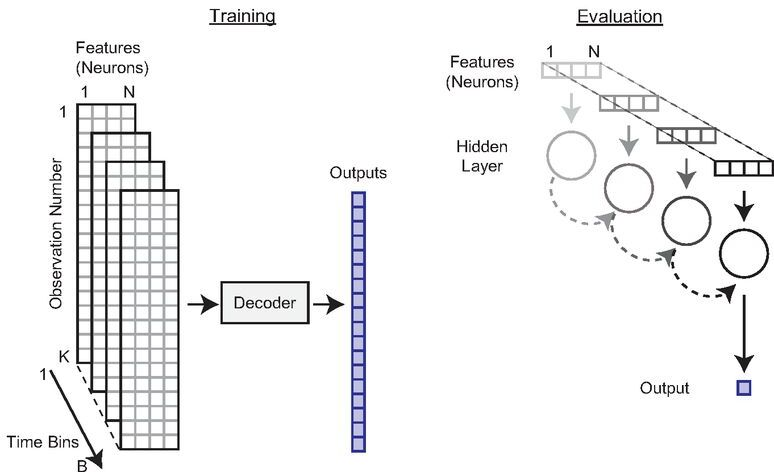
\includegraphics[width=\textwidth]{rnn-schema.jpg}
		\caption{Схема обучения и предсказания рекуррентного декодера. Взято из \citep{glaser2020machine}}
		\label{fig:rnn-schema}
	\end{figure}

	Cвойства: количество параметров = $K^2 + Ks + Kd = O(KM)$, время прямого прохода = $O(KML)$

	Преимущества: есть реализация во всех фреймворках глубокого обучения, относительно быстрое обучение и предсказание модели

	Недостатки: не работают с данными, содержащими пропуски и/или разной частотой сэмплирования

	\subsection{Нейронные контролируемые дифференциальные уравнения (NCDE)}
	В модели нейронных обыкновенных дифференциальных уравнений (NODE), прародителе модели NCDE, предполагается, что скрытое состояние описывается дифференциальным уравнением \ref{eq:node}.
	
	\begin{equation}\label{eq:node}
		\bx'(t) = \bff(\bw, \bx(t))
	\end{equation}

	Данный подход позволяет более качественно описывать временной ряд, порождённый динамической системой. Предсказание модели получаются решением дифференциально-
	го уравнения \ref{eq:node} с начальными условиями, в котором правая часть задается нейронной сетью. Это означает, что за один прямой проход алгоритм выдает всю траекторию, в отличие от рекуррентных сетей.
	
	Однако у модели NODE есть и минусы.
	Во-первых, выдаваемое ею решение дифференциального уравнения зависит только от начального состояния, которое постоянно во времени.
	Во-вторых, не существует механизма для дообучения модели на основе новых данных.
	Эти пробелы нивелируются моделью нейронных контролируемых дифференциальных уравнений, представленной уравнением \ref{eq:ncde}.
	
	\begin{equation}\label{eq:ncde}
		\begin{aligned}
			\bx(t_1) &= \zeta(\bu_1, t_1) \\
			\bx(t) &= \bx(t_1) + \int_{t_1}^t \bff(\bx(\tau))dU(\tau) \\
			\by_i &= g(\bx(t_i))
		\end{aligned}
	\end{equation}
	$\text{где } \bu_i \in \dR^d, \; \by_i \in \dR^s $
	
	$\bx: [t_1, t_L] \rightarrow \dR^K$ ~--- функция скрытого состояния
	
	$U: [t_1, t_L] \rightarrow \dR^{d+1}$ ~--- кубический сплайн 
	
	$\zeta: \dR^{d+1} \rightarrow \dR^K$ ~--- проектор в скрытое пространство
	
	$f: \dR^K \rightarrow \dR^{K \times (d+1)}$ ~--- динамика скрытого состояния

	$g: \dR^K \rightarrow \dR^s$ ~--- линейное отображение
	
	Теперь, начальное состояние модели NCDE содержит информацию о времени наблюдения первого объекта.
	При решении дифференциального уравнения в интегральной форме используется интеграл Римана-Стильтьесса вместо интеграла Римана, агрегируя таким образом все наблюдения.
	Высокоуровневый план модели NCDE изображён на рисунке \ref{fig:ncde}.
	
	\begin{figure}[bhtp]
		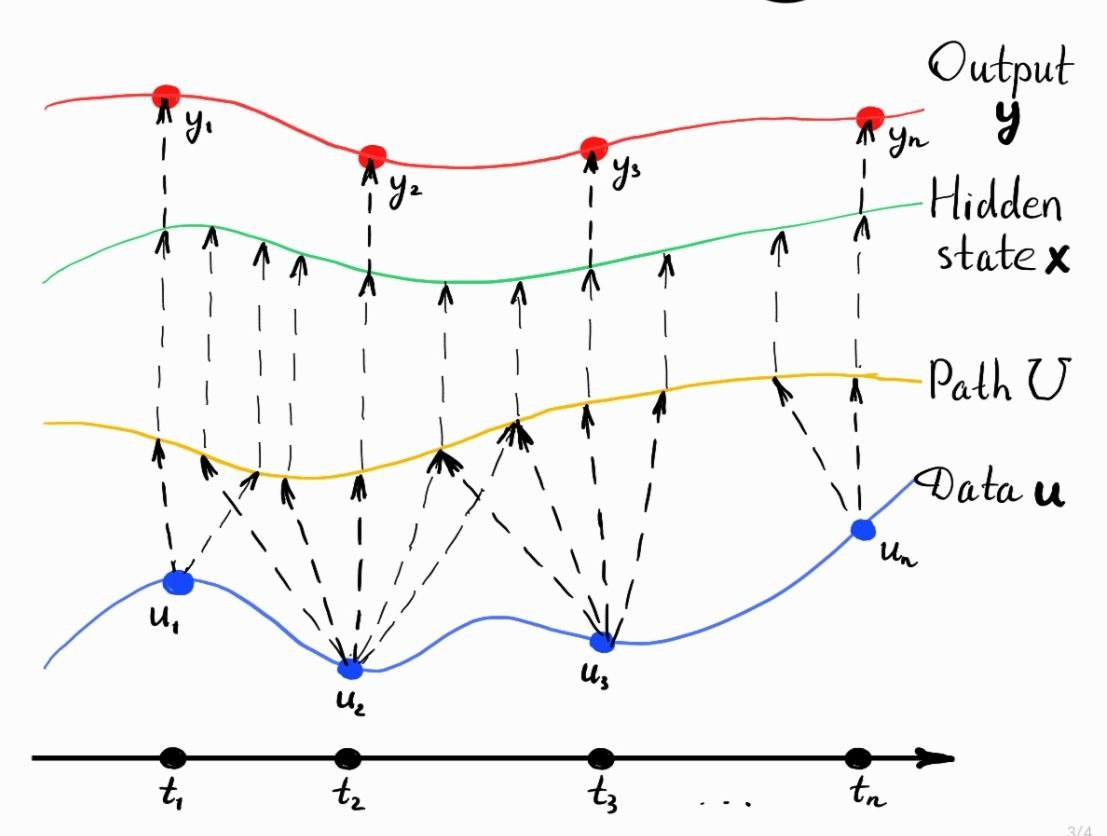
\includegraphics[width=\textwidth]{neural-cde-path.jpg}
		\caption{Иллюстрация алгоритма Neural CDE}
		\label{fig:ncde}
	\end{figure}
	
	Уделим особое внимание пути $U(t)$, модифицируя который можно получать разные модели:
	\begin{itemize}
		\item $U(t) = t$ ~--- модель Neural ODE \citep{node}
		\item $U(t) = \sum\limits_{i=1}^{L-1} \bu_{t_i} \cdot I(t_i \leqslant t < t_{i+1})$ ~--- модель ODE-RNN \citep{latent-ode}
		\item $U(t) = \sum\limits_{i=1}^{L-1} \alpha_i(t) \bu_{t_i} + (1-\alpha_i(t)) \bu_{t_{i+1}} \cdot I(t_i \leqslant t < t_{i+1}), \text{где } \alpha_i(t) = \dfrac{t_{i+1} - t}{t_{i+1} - t_i}$ ~--- модель c линейной функцией интерполяции
	\end{itemize}

	Дообучать модель NCDE можно, решая интегральное уравнение с момента $t_{L}$.
	Однако, данная опция доступна не для всех функций пути: для кубического сплайна ~--- нельзя, а для остальных перечисленных ~--- можно.
	Связано это с тем, что при получении новых данных, старый путь может оказаться невалиден, вследствие чего невалидным окажется и состояние $\bx(t_L)$ \citep{ncde-online}. 
	
	Но и у модели Neural CDE есть недостаток: это большое количество параметров, используемых в функции $\bff$.
	Если в качестве $\bff$ использовать линейную функцию, то число параметров равняется $O(K^2d)$, что на порядок больше, чем у RNN.
	В оригинальной статье \citep{ncde} авторы использовали линейную функцию с малым $K$.
	Также можно использовать малоранговое линейное преобразование, использующее $O(K^2 + Kd)$ параметров, но в статье \citep{ncde} показана неэффективность данного подхода.
	
	Cвойства: количество параметров = $O(K^2d + Ks)$, время прямого прохода = $O(K^2dL)$
	
	Преимущества: работает с данными, в которых содержатся пропуски и которые имеют разную частоту сэмплирования, большая гибкость в настройке модели: выбор архитектуры функции $\bff(\bx)$ и пути $U(t)$
	
	Недостатки: в десятки раз медленнее, чем RNN, на текущий момент не существует эффективной реализации, долгая настройка модели, нестабильное обучение при больших $K$, при использовании солверов с адаптивным шагом и функции активации ReLU

	\subsection{Модель структурированного пространства состояний (S4)}
	Данная модель строится из модели пространства состояний в 3 шага. Во-первых, применяется билинейное преобразование для перехода из непрерывной постановки \ref{eq:ssm-cont} в дискретную \ref{eq:ssm-discr} со следующими характеристиками:
	\begin{align*}
		&u_i = u(i\Delta) \\
		&\overline{A} = (I - \dfrac{\Delta}{2} A)^{-1} (I + \dfrac{\Delta}{2} A) \\
		&\overline{B} = (I - \dfrac{\Delta}{2} A)^{-1} \Delta B \\
		&\overline{C} = C \\
		&\overline{D} = 0
	\end{align*}
	где $\Delta$ ~--- шаг дискретизации.
	
	Далее переходим к свёрточному представлению модели \ref{eq:ssm-discr} с вышеуказанными параметрами. Делается это из соображений эффективности по времени.
	\begin{equation*}
		\begin{split}
			\bx_0 &= \overline{B}\bu_0 \\
			\bx_1 &= \overline{A}\overline{B}\bu_0 + \overline{B}\bu_1 \\
			\bx_2 &= \overline{A}^2\overline{B}\bu_0 + \overline{A}\overline{B}\bu_1 + \overline{B}\bu_2 \\
			\cdots 
		\end{split}
		\qquad
		\begin{split}
			\by_0 &= \overline{C}\overline{B}\bu_0 \\
			\by_1 &= \overline{C}\overline{A}\overline{B}\bu_0 + \overline{C}\overline{B}\bu_1 \\
			\by_2 &= \overline{C}\overline{A}^2\overline{B}\bu_0 + \overline{C}\overline{A}\overline{B}\bu_1 + \overline{C}\overline{B}\bu_2 \\
			\cdots 
		\end{split}
	\end{equation*}
	\begin{equation*}
		\begin{split}
			\by_i &= \overline{C}\overline{A}^i\overline{B}\bu_0 + \overline{C}\overline{A}^{i-1}\overline{B}\bu_1 + \ldots + \overline{C}\overline{A}\overline{B}\bu_{i-1} + \overline{C}\overline{B}\bu_i \\
			\by &= \overline{\mathbf{K}} \ast \bu, \text{ где } \overline{\mathbf{K}} = (\overline{C}\overline{B}, \overline{C}\overline{A}\overline{B}, \ldots, \overline{C}\overline{A}^{L-1}\overline{B}) 
		\end{split}
	\end{equation*}

	Таким образом, если ядро свёртки $\overline{\mathbf{K}}$ уже предпосчитано, то можно быстро применить данный слой.
	Однако для матрицы $A$ общего вида вычисление займёт $O(LK^2)$ памяти и $O(LK^3)$ времени (при $d=s=1$).
	Для экономии памяти вместо ядра свёртки хранятся значения производящей функции от данной последовательности в корнях степени $L$ от 1.
	Для уменьшения же временных затрат на матрицу $A$ накладывают ограничения ~--- она должна иметь следующий вид:
	$$ A = \Lambda - PQ^*,$$
	где $\Lambda \in \dR^{K \times K}$ ~--- диагональная матрица, $P, Q \in \dR^{K \times 1}$
	
	И в третьих, с помощью инициализации HIPPO получаются начальные приближения для $\Lambda, P, Q$.
	Инициализация HIPPO имеет следующий вид:
	\begin{equation*}
		A_{nk} = -
		\begin{cases}
			\sqrt{(2n+1)(2k+1)} &\text{ при } n > k \\
			n+1 &\text{ при } n = k \\
			0 &\text{ при } n < k \\
		\end{cases}
	\end{equation*}

	
	Подробную информацию о каждом шаге можно найти в работе \citep{s4}.
	
	Cвойства: количество параметров = $Kd + Ks$, время прямого прохода = $O(KML)$

	Преимущества: хорошо работает с данными, содержащими долговременные зависимости, есть эффективная реализация \citep{s4-git}
	
	Недостатки: не работают с данными, содержащими пропуски и/или разной частотой сэмплирования
		
	\subsection{Сравнение моделей}
	В таблице \ref{tbl:dl-analysis} приведено описание свойств различных моделей глубокого обучения. Помимо моделей пространства состояний, для полноты картины указаны свёрточные нейронные сети и трансформеры.
	
	Для CNN используются другие обозначения: $K$ ~--- размер ядра свёртки, $Ch$ ~--- количество каналов ЭКоГ. Считаем, что количество каналов в свёртке равняется одному и что размер ядра свёртки составляет $K \times K$
	
	\begin{table}[bhtp]
		\centering
		\caption{Сравнение моделей по числу обучаемых параметров, времени прямого прохода, наличию эффективной реализации, возможности работы с пропусками и хранения всей истории}
		\label{tbl:dl-analysis}
		\begin{tabularx}{0.95\textwidth}{c|c|c|X|X|X|}
			\cline{2-6}
			\multicolumn{1}{l|}{}             & Parameters & Forward & Fast impl. & Cont. time & Unb. context \\ \hline
			\multicolumn{1}{|c|}{RNN}         & $O(KM)$ & $O(KML)$ & $+$ & $-$ & $+$ \\ \hline
			\multicolumn{1}{|c|}{NCDE}  & $O(K^2d + Ks)$ & $O(K^2dL)$ & $-$ & $+$ & $+$ \\ \hline
			\multicolumn{1}{|c|}{S4}          & $O(Kd + Ks)$ & $O(KML)$ & $+$ & $-$ & $+$ \\ \hline
			\multicolumn{1}{|c|}{Transformer} & $O(K^2d + Ks)$ & $O(LK \cdot (L+s))$ & $+$ & $-$ & $+$ \\ \hline
			\multicolumn{1}{|c|}{CNN} & $O(K^2)$ & $O(K^2(L-K)(N-K))$ & $+$ & $-$ & $-$ \\ \hline
		\end{tabularx}
	\end{table}

	
	%%%%%%%%%%%%%%%%%%%%%%%%%%%%%%%%%%%%%%%%%%%%%%%%%%%%%%%%%%%%%%%%%%%%%%%%%%%%%%%%%%%%%%%%%%%%%%%%%%%%%%%%%%%%%%%%%%%%%%%%%%%%%%%%
	\section{Вычислительный эксперимент}
	Целью эксперимента является сравнение ранее перечисленных методов пространства состояний. 
	Эти методы применяются для предсказания наличия стимула по сигналам головного мозга.
	
	\subsection{Экспериментальные данные}
	Одновременные ЭКоГ-записи были получены от 12 участников (8 мужчин, 4 женщины)
	в ходе непрерывного клинического мониторинга эпилепсии, проводимого в медицинском центре Харборвью в Сиэтле.
	Эти записи длятся 7 $\pm$ 2 дня на каждого участника. Возраст участников составляет 29 $\pm$ 8 лет, и им были имплантированы электроды, преимущественно в одно полушарие (5 правых, 7 левых).
	
	Задача декодирования заключается в том, чтобы классифицировать события "движения" и "покоя" верхней конечности руки, противоположной полушарию имплантированного электрода.
	События перемещения соответствуют движению запястья, которое произошло по крайней мере через 0.5 с без движения, в то время как события покоя указывают на отсутствие движения ни в одном запястье в течение по крайней мере 3 с.
	
	Обработка данных ECoG осуществлена с использованием обычных скриптов MNE-Python. 
	Сначала был удалён средний дрейф постоянного тока и высокоамплитудные разрывы. Затем данные ECoG каждого участника подвергались полосовой фильтрации (1-200 Гц), notch-фильтрации и повторной привязке к общей медиане по электродам. 
	Также удалены зашумлённые сигналы на основе аномального стандартного отклонения (> 5 МКР) или эксцесса (> 10 МКР). 
	Затем сгенерированны 10-секундные сегменты ECoG, сосредоточенные вокруг каждого события "движение" и "отдых". 
	Сегменты ECoG с отсутствующими данными или большими артефактами были удалены на основе аномальной спектральной плотности мощности \citep{peterson2021behavioral}.
	Затем частота сигнала была уменьшена до 250 Гц, а временные интервалы сокращены до 2 секунд по центру каждого события.
	Для каждого участника было сбалансировано количество сегментов движения и отдыха в течение каждого дня записи, в результате чего на одного участника пришлось 1155 $\pm$ 568 событий.
	
	\subsection{Условия проведения эксперимента}
	\begin{figure}[bhtp]
		\centering
		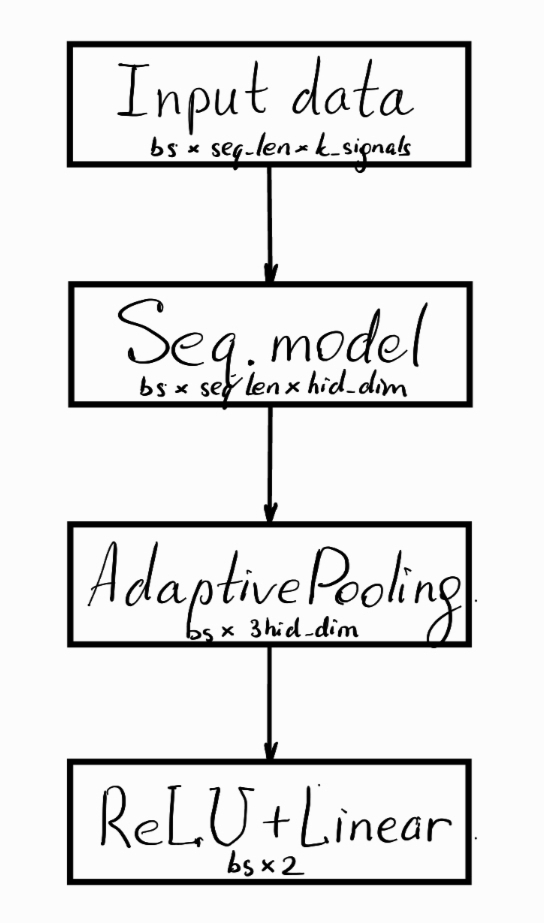
\includegraphics[height=9cm]{seq-model.jpg}
		\caption{Архитектура модели классификации}
		\label{fig:seq-model}
	\end{figure}
	
	Структура модели декодирования сигнала ЭКоГ приведена на рисунке \ref{fig:seq-model}.
	Вначале применяется модель пространства состояний, затем идёт агрегирующий слой, который по каждому элементу и каналу берёт максимум, среднее и последний элемент, после идёт функция активации ReLU и линейное преобразование.
	
	Ввиду переобучения моделей, в Seq.model внедрён SpatialDropout, который зануляет сразу весь канал, а не его случайные элементы.
	
	Участники разбиваются на обучающую, валидационную и тестовую выборки в соотношении $7-4-1$. Модель обучается 20 раз, каждая на одном из 20 разбиений, результаты предсказания затем усредняются.
	
	В качестве рекуррентной нейронной сети используется LSTM, в Neural CDE используются кубические сплайны с методом Рунге-Кутты 4го порядка. 
	
	Константы: $\lambda = 0.002$ (L2-регуляризация), p = 0.5 (dropout), batch size = 32, hidden size = 32, оптимизатор = AdamW с lr = 0.002, 
	
	\subsection{Анализ ошибки}
	\begin{figure}[bhtp]
		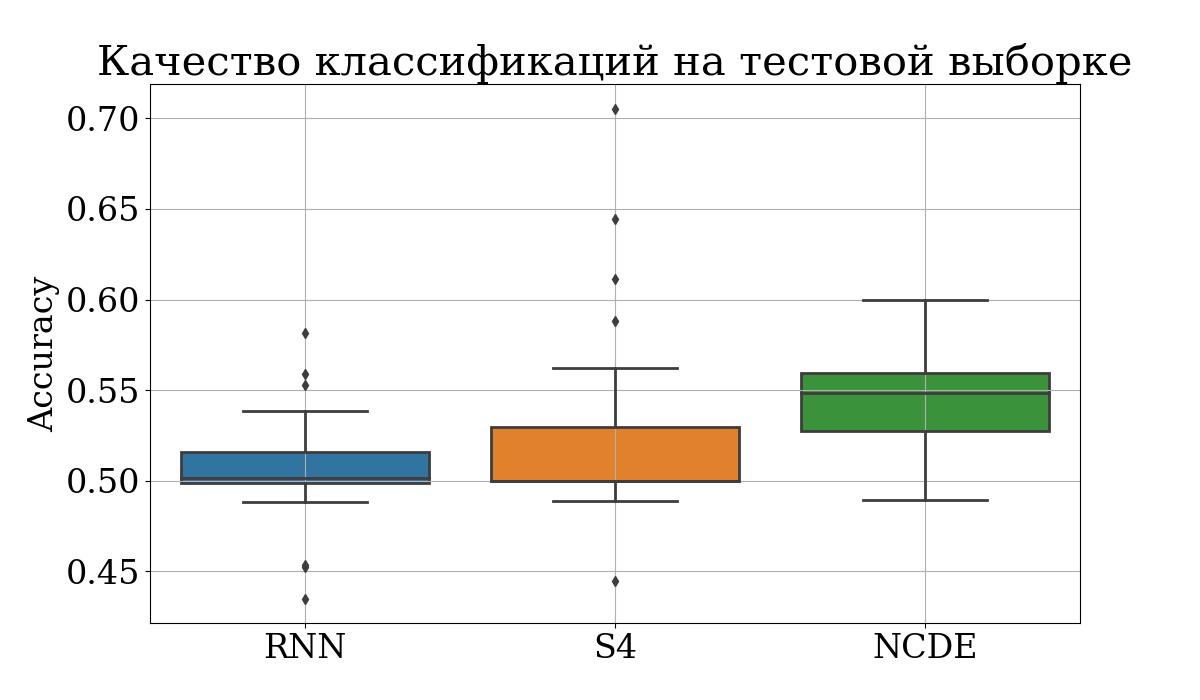
\includegraphics[width=\textwidth]{rnn-s4-ncde.png}
		\caption{Точность предсказания моделей пространства состояний}
		\label{fig:accuracy-analysis}
	\end{figure}

	Результаты обучения моделей показаны на рисунке \ref{fig:accuracy-analysis} и в  таблице \ref{tbl:rnn-s4-ncde}. Видим, что accuracy всех моделей чуть выше 0.5, с учётом равномерного распределения классов это говорит о низком качестве предсказания. Связано это с тем, что модель не выучила "хорошее" признаковое представление сигналов. В таких случаях принято использовать CNN для извлечения "полезных" признаков и увеличения качества прогноза.
	Исходя из полученных результатов, можно заключить, что Neural CDE имеет лучшую точность предсказания на тестовой выборке. Но время обучения превышает время RNN почти в 8 раз.

	\begin{table}[bhtp]
		\centering
		\caption{Сравнение характеристик RNN, S4 и NCDE}
		\label{tbl:rnn-s4-ncde}
		\begin{tabular}{c|l|l|l|}
			\cline{2-4}
			\multicolumn{1}{l|}{}  & Parameters & Time per epoch (sec) & Accuracy \\ \hline
			\multicolumn{1}{|c|}{RNN} & 45.5k & $3.42 \pm 0.55$ & 0.516 $\pm$ 0.027 \\ \hline
			\multicolumn{1}{|c|}{S4} & 38k & $3.12 \pm 0.81$ & 0.591 $\pm$ 0.049 \\ \hline
			\multicolumn{1}{|c|}{Neural CDE} & 153.3k & $37.23 \pm 0.64$ & 0.596 $\pm$ 0.026 \\ \hline
		\end{tabular}
	\end{table}
	
	\subsection{Итоговые рекомендации}
	Предлагается использовать модели семейства RNN в качестве начального подхода. Далее, если длина последовательности слишком большая (порядка 10 тысяч) или если требуется получить более высокое качество предсказания, то стоит приглядеться к модели S4. Затем, если в данных есть пропущенные значения, а при текущем методе заполнения пропусков (например, средним или константой) качество предсказания по-прежнему невысокое, или если частота сэмплирования непостоянна во времени, то нужно применить модель Neural CDE. Отдельного внимания заслуживает выбор функции пути. В случае, если необходимо делать прогнозы в режиме онлайн, то подойдут прямолинейная и линейная интерполяции. Иначе, стоит выбрать кубические сплайны. Однако нужно учесть, что время обучения данной модели в десятки раз больше, чем у рекуррентных нейронных сетей. Также случаются провалы в работе модели с настройками по умолчанию, так что придётся уменьшать максимальное значение ошибки, менять решатель дифференциального уравнения и архитектуру модели.
	
	%%%%%%%%%%%%%%%%%%%%%%%%%%%%%%%%%%%%%%%%%%%%%%%%%%%%%%%%%%%%%%%%%%%%%%%%%%%%%%%%%%%%%%%%%%%%%%%%%%%%%%%%%%%%%%%%%%%%%%%%%%%%%%%%%%%%%%%
	\section{Заключение}
	Рассмотрено применение моделей пространства состояний в задаче классификации сигналов ЭКоГ.
	Изучены свойства следующих моделей пространства состояний: RNN, NCDE, S4.
	Предоставлена рекомендация по выбору моделей пространства состояния.
	Продемонстрировано, что модель Neural CDE имеет лучшее качество на тестовой выборке по сравнению с другими моделями, однако её время обучения сильно превышает время обучения других моделей.
	
	%%%%%%%%%%%%%%%%%%%%%%%%%%%%%%%%%%%%%%%%%%%%%%%%%%%%%%%%%%%%%%%%%%%%%%%%%
	\addcontentsline{toc}{section}{\protect\numberline{}Список литературы}
	\bibliographystyle{unsrtnat}
	\bibliography{references.bib}
	
\end{document} 